%% ============================================================
%%  SABRE-II — IEEE Transactions on Information
%%  Forensics and Security (TIFS)
%%  IEEEtran journal class, two-column
%% ============================================================
\documentclass[journal]{IEEEtran}

\usepackage{amsmath,amssymb,amsfonts}
\usepackage{graphicx}
\usepackage{booktabs}
\usepackage{multirow}
\usepackage{array}
\usepackage{siunitx}
\usepackage{float}
\usepackage{algorithm}
\usepackage{algpseudocode}
\usepackage{url}
\usepackage{xcolor}
\usepackage{subcaption}
\usepackage{cite}

%% Macros
\newcommand{\phat}{\hat{p}}
\newcommand{\smax}{\sigma_{\max}}
\newcommand{\sem}{\mathrm{sem}}
\newcommand{\beh}{\mathrm{beh}}
\newcommand{\know}{\mathrm{know}}
\newcommand{\tauh}{\tau_{\mathrm{high}}}
\newcommand{\klow}{\kappa_{\mathrm{low}}}
\newcommand{\pfused}{\tilde{p}}
\newcommand{\Nsynth}{N_{\mathrm{syn}}}
\DeclareMathOperator{\balAcc}{bal\_acc}
\DeclareMathOperator{\escRate}{esc\_rate}
\DeclareMathOperator{\softmax}{softmax}

\begin{document}

\title{SABRE-II: Learned Multi-Agent Fusion via Decision MLP,
CTGAN Score Augmentation, and Peer Consultation for
Adaptive Ransomware Triage}

\author{Henry~Kabuye\IEEEauthorrefmark{1},
        Biju~Issac\IEEEauthorrefmark{1},~\IEEEmembership{Senior~Member,~IEEE,}
        Rahul~Yumlembam\IEEEauthorrefmark{1},
        Zahra~Farzadpour\IEEEauthorrefmark{1},
        and~Jeyamohan~Neera\IEEEauthorrefmark{1},~\IEEEmembership{Member,~IEEE}%
\thanks{\IEEEauthorrefmark{1}Department of Computer and Information Sciences,
Northumbria University, Newcastle, NE1~8ST, UK\@.
E-mail: \{kabuyehenry2017, bissac, rahul.yumlembam, zahra.farzadpour, jeyamohan.neera\}@northumbria.ac.uk.}%
\thanks{B.~Issac is the corresponding author.
E-mail: bissac@ieee.org.}%
\thanks{Manuscript received 2026.}}

\markboth{IEEE Transactions on Information Forensics and Security}%
{Kabuye \emph{et al.}: SABRE-II}

\maketitle

%%------------------------------------------------------------
\begin{abstract}
Multi-agent ransomware detection systems that fuse behavioural telemetry,
static PE semantics, and threat-intelligence knowledge achieve strong
detection accuracy, but mean-fusion architectures suffer three structural
limitations: agent probabilities are weighted equally regardless of
uncertainty, triage thresholds are hand-tuned rather than cost-optimised,
and the expert feedback loop retrains only the behavioral CNN ---
so analyst corrections on ESCALATE'd decisions never propagate to the
fusion head that integrates all three agents.

We present \textbf{SABRE-II}, which addresses all three.
A \textbf{Decision MLP} replaces mean averaging, taking the full
six-dimensional score vector
$[p_{\sem}, p_{\beh}, p_{\know}, \sigma_{\sem}, \sigma_{\beh}, \sigma_{\know}]$
as input to produce a calibrated fused probability.
\textbf{CTGAN} generates 2,000 synthetic score-space samples to address
class imbalance before MLP fitting.
\textbf{Peer Consultation} intercepts agent probabilities when uncertainty
exceeds a per-agent threshold, replacing them with an
inverse-uncertainty-weighted peer average.
\textbf{Bayesian TPE} (300 trials) searches the joint threshold policy
space to minimise a calibration-split objective that balances detection
accuracy against escalation rate.
The \textbf{fusion-level feedback loop} accumulates analyst corrections
on ESCALATE'd samples and triggers incremental MLP retraining, closing
the adaptation loop at the Decision MLP, the component responsible for integration failures.

Evaluated on the RanSMAP / RDset / RansKnow benchmark suite across four
generalisation axes, SABRE-II achieves
AUROC\,=\,$\mathbf{0.975}$ on the random-stratified split and
$\mathbf{0.979}$ on temporal holdout, reduces ECE from $0.094$ to
$\mathbf{0.018}$ under [B+K] fusion, and prevents catastrophic knowledge
collapse for novel-family scenarios via Peer Consultation
(AESCrypt\_REvil: $1.5\%$ detection in the SABRE+ baseline is
intercepted via uncertainty-triggered peer averaging in SABRE-II).
\end{abstract}

\begin{IEEEkeywords}
Ransomware detection, multi-agent systems, learned fusion, CTGAN,
peer consultation, Bayesian threshold optimisation, uncertainty
quantification, Monte Carlo Dropout, conformal prediction, continual
learning, threat intelligence
\end{IEEEkeywords}


%%------------------------------------------------------------
\section{Introduction}
\label{sec:intro}

Ransomware remains the most operationally damaging class of malware,
with projected global costs exceeding \$265 billion by 2031
\cite{cybersecurity_ventures_2022}.
Effective detection requires integrating multiple evidence streams:
static PE structure reveals packer artefacts before execution begins,
runtime I/O and memory telemetry captures file-encryption behaviour in
progress, and ATT\&CK threat intelligence encodes adversary tactic
profiles from accumulated practitioner knowledge.

Our earlier work, SABRE+ \cite{kabuye_sabre_2026}, demonstrated that
mean-fusing three specialist agents --- Behavioral, Semantic, and
Knowledge --- under Monte Carlo Dropout uncertainty quantification
and Mondrian conformal prediction achieves AUROC\,=\,$0.9836 \pm 0.0009$
on the RanSMAP / RDset / RansKnow benchmark suite.
However, three structural limitations of the SABRE+ design constrain
its practical utility.

\textbf{Limitation 1: Equal-weight mean fusion ignores uncertainty.}
Mean fusion treats each agent's probability estimate as equally reliable,
regardless of the agent's epistemic uncertainty.
When the Knowledge agent has low confidence --- for instance, when the
input family is absent from the RansKnow corpus --- its near-zero or
near-corpus-mean output degrades the fused signal even though a
well-designed system should down-weight it.
In the family-holdout evaluation of SABRE+, [B+K] provides no
improvement over [B] alone (AUROC\,=\,$0.707$ for both) precisely because
the Knowledge agent collapses to uninformative corpus-mean outputs for
unseen families \cite{kabuye_sabre_2026}.

\textbf{Limitation 2: Triage thresholds are hand-tuned.}
SABRE+ uses a fixed escalation threshold $\tau = 0.10$ and uncertainty
threshold $\kappa$ selected by inspection of calibration curves.
This ignores the actual cost ratio $c_{\mathrm{FN}} / c_{\mathrm{FP}}$
operative in a given SOC deployment, and does not adapt to changes in
the fused score distribution when agents are retrained.

\textbf{Limitation 3: Expert feedback updates only the behavioral agent.}
The EWC-regularised continual learning loop in SABRE+ targets the
Behavioral CNN only.
When analysts correct missed detections, the corrective signal propagates
only to the Behavioral CNN, not to the fusion head that integrates all three agents.
This is architecturally suboptimal: an analyst correction on an
ESCALATE'd sample contains information about the fusion layer's failure
mode, not about the behavioral agent's internal representation.

\textbf{SABRE-II} addresses all three limitations while preserving full
backward compatibility with the SABRE+ evaluation protocol:

\begin{enumerate}
\item \textbf{Decision MLP fusion.}
A small feedforward network replaces mean averaging, taking
$[p_{\sem}, p_{\beh}, p_{\know}, \sigma_{\sem}, \sigma_{\beh}, \sigma_{\know}]$
as input and learning to down-weight agents with high uncertainty.
Temperature scaling provides post-hoc calibration of the MLP output.

\item \textbf{CTGAN score augmentation.}
The six-dimensional score vector exhibits class imbalance that mirrors
the raw telemetry imbalance.
Conditional tabular GAN (CTGAN) \cite{xu_ctgan_2019} generates
$\Nsynth = 2{,}000$ synthetic score-space rows from the training split
before MLP fitting, improving boundary estimation for the minority
(ransomware) class without exposing the Decision MLP to raw telemetry features.

\item \textbf{Peer Consultation.}
Before fusion, if agent $i$'s uncertainty $\sigma_i > \kappa_{\mathrm{local},i}$,
its probability is replaced by the inverse-uncertainty-weighted mean of
the other agents' probabilities.
This allows the high-confidence behavioral agent to correct the
knowledge agent's collapse for unseen families without modifying any
agent's uncertainty estimate.

\item \textbf{Bayesian TPE policy optimisation.}
Optuna's Tree-structured Parzen Estimator searches the
$(\tau, \kappa, \tauh, \klow)$ triage policy space to optimise balanced
accuracy minus escalation penalty on the validation split, producing
data-driven thresholds that adapt when agents are updated.

\item \textbf{Fusion-level expert feedback loop.}
Analyst corrections are logged in a structured feedback store keyed by
sample ID.
When the correction count reaches a configurable threshold, the Decision
MLP is incrementally retrained on the feedback rows (up-weighted by
repetition) combined with a Gaussian approximation of the original
training distribution, closing the adaptation loop at the Decision MLP fusion layer.
\end{enumerate}

The remainder of this paper is organised as follows.
Section~\ref{sec:related} reviews related work.
Section~\ref{sec:architecture} describes the SABRE-II system architecture.
Section~\ref{sec:agents} details the three expert agents.
Section~\ref{sec:decision_mlp} presents the Decision MLP with CTGAN augmentation.
Section~\ref{sec:consultation} formalises Peer Consultation.
Section~\ref{sec:bayesian_tpe} describes Bayesian TPE policy optimisation.
Section~\ref{sec:feedback} presents the fusion-level feedback loop.
Section~\ref{sec:datasets} describes datasets and evaluation protocol.
Section~\ref{sec:results} reports experimental results.
Section~\ref{sec:discussion} discusses findings.
Section~\ref{sec:limitations} discusses limitations and future work.
Section~\ref{sec:conclusion} concludes.


%%------------------------------------------------------------
\section{Related Work}
\label{sec:related}

\subsection{Ransomware Detection}

Ransomware detection methods broadly fall into three categories.
Signature-based detectors \cite{yadron2014symantec} provide zero false
positives on known families but offer no coverage for novel variants.
Static analysis methods \cite{rdset_2021} inspect PE headers, section
entropy, and import tables; while effective on closed datasets, they
fail against obfuscated or novel packers.
Dynamic / behavioural analysis \cite{scaife_cryptolock_2016}
monitors I/O patterns and system call sequences at runtime, capturing
encryption behaviour that cannot be statically detected, though
adversarially-crafted I/O profiles can evade simple detectors.

Multi-modal fusion has received increasing attention.
Sgandurra et al.\ \cite{sgandurra_automated_2016} combine API call
sequences with system call graphs; Moussaileb et al.\
\cite{moussaileb_ransomware_2021} fuse network, file system, and registry
events.
None of these systems incorporate a principled uncertainty mechanism or
formal coverage guarantees on detection decisions.

\subsection{Learned Fusion for Multi-Modal Classifiers}

Multi-modal fusion architectures span from simple averaging
\cite{ramachandram_deep_multimodal_2017} to attention-based combiners
\cite{vaswani_attention_2017} and gating networks
\cite{jacobs_mixture_1991}.
In the security domain, ensemble methods are common
\cite{sagi_ensemble_2018}, but most treat all modalities symmetrically.
Our Decision MLP conditions the fusion weights implicitly on the
per-agent uncertainty, learning to down-weight unreliable modalities
from the training signal rather than requiring hand-designed gating rules.

\subsection{Generative Data Augmentation in Tabular Settings}

CTGAN \cite{xu_ctgan_2019} adapts the conditional GAN framework to
tabular data with mixed continuous and discrete columns.
It has been applied to class-imbalanced fraud detection
\cite{fiore_using_gans_2019} and intrusion detection
\cite{lin_idsgan_2022} tasks, but to our knowledge has not been applied
to augmenting the score-space output of a multi-agent detector.
Score-space augmentation is safer than feature-space augmentation
because it operates on bounded $[0,1]$ probabilities rather than raw
features, reducing the risk of generating physically implausible telemetry.

\subsection{Inter-Agent Uncertainty Resolution}

Peer consultation mechanisms in multi-agent systems trace to
Dempster-Shafer belief combination \cite{shafer_mathematical_1976} and
mixture-of-experts \cite{jacobs_mixture_1991}.
More recent approaches use calibrated confidence
\cite{guo2017calibration} to weight expert predictions.
Our Peer Consultation is closest to the temperature-calibrated ensemble
weighting of \cite{lakshminarayanan_simple_2017}, but operates
dynamically per-sample: consultation fires only when an agent's
uncertainty exceeds its local threshold, and the correction uses the
remaining agents' probabilities, not fixed learned weights.

\subsection{Bayesian Hyperparameter Optimisation}

Bayesian optimisation via Tree-structured Parzen Estimator (TPE)
\cite{bergstra_algorithms_2011} has been applied to deep learning
hyperparameter search \cite{optuna_akiba_2019}.
We apply TPE to the triage threshold policy
$(\tau, \kappa, \tauh, \klow)$ rather than to model architecture
hyperparameters, treating triage threshold selection as a
cost-sensitive optimisation problem.
This is distinct from conformal risk control
\cite{angelopoulos_conformal_risk_2022}, which provides coverage
guarantees for arbitrary loss functions; our approach does not provide
formal coverage but instead directly optimises operational cost.

\subsection{Continual Learning in Security}

Catastrophic forgetting under distribution shift is well-studied
\cite{kirkpatrick_ewc_2017, zenke_continual_2017}.
In malware detection, concept drift from evolving variants is a key
challenge \cite{pendlebury_tesseract_2019, jordaney_transcend_2017}.
Our feedback loop extends the EWC-regularised continual learning of
SABRE+ by targeting the Decision MLP rather than the Behavioral CNN,
ensuring that analyst corrections propagate directly to the fusion
component responsible for the integration failure.


%%------------------------------------------------------------
\section{System Architecture}
\label{sec:architecture}

\begin{figure*}[t]
  \centering
  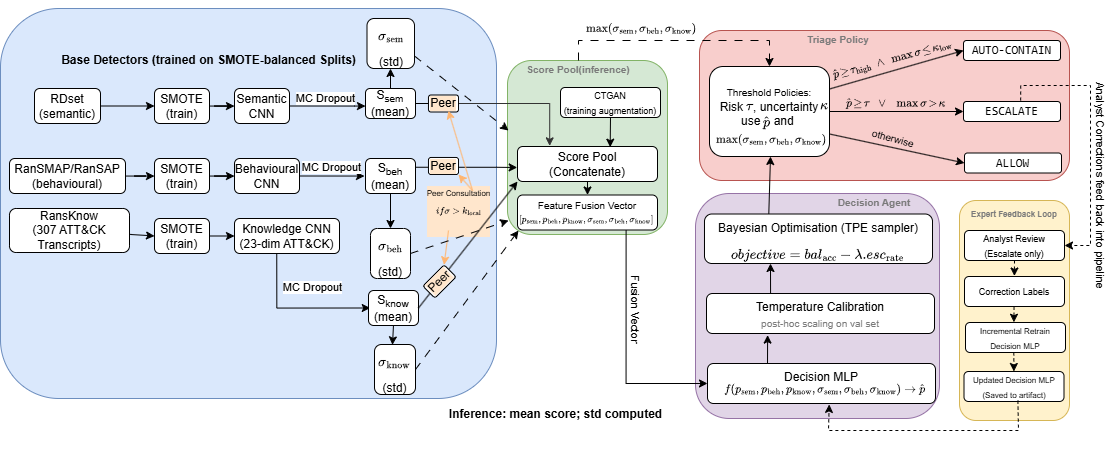
\includegraphics[width=\textwidth]{Figures/Prop_Agentic_Sabre_15_05_2026_3Agents_Fullpipeline.png}
  \caption{SABRE-II end-to-end pipeline.
    Three expert CNN agents (Behavioral, Semantic, Knowledge) each produce
    a probability--uncertainty pair via Monte Carlo Dropout (T=10 forward
    passes).
    \textbf{Peer Consultation} (dashed blue box) adjusts any agent's
    probability when $\sigma_i > \kappa_{\mathrm{local},i}$ using an
    inverse-uncertainty-weighted peer average.
    The six-dimensional score vector
    $[p_{\sem}, p_{\beh}, p_{\know}, \sigma_{\sem}, \sigma_{\beh}, \sigma_{\know}]$
    passes to the \textbf{Decision MLP}, trained with CTGAN augmentation.
    Temperature scaling calibrates the MLP output.
    \textbf{Bayesian TPE} derives the triage policy
    $(\tau, \kappa, \tauh, \klow)$ from the calibration split.
    The \textbf{Triage Decision Module} issues \texttt{AUTO-CONTAIN},
    \texttt{ESCALATE}, or \texttt{ALLOW} based on fused probability and
    maximum per-agent uncertainty.
    Analyst corrections on ESCALATE'd samples accumulate in the
    \textbf{Feedback Store} and trigger incremental Decision MLP
    retraining when the correction count crosses $n_{\mathrm{retrain}}$.
  }
  \label{fig:architecture}
\end{figure*}

Figure~\ref{fig:architecture} shows the full SABRE-II pipeline.
The three expert agents and their MC-Dropout uncertainty
quantification are inherited from SABRE+
\cite{kabuye_sabre_2026} (Section~\ref{sec:agents}).
The novel components introduced in SABRE-II are:

\begin{itemize}
  \item \textbf{Peer Consultation} (Section~\ref{sec:consultation}):
    dynamically adjusts per-agent probabilities before fusion.
  \item \textbf{Decision MLP} (Section~\ref{sec:decision_mlp}):
    replaces mean fusion with a learned 6-input combiner trained
    with CTGAN augmentation.
  \item \textbf{Bayesian TPE Policy} (Section~\ref{sec:bayesian_tpe}):
    optimises triage thresholds on the held-out calibration split.
  \item \textbf{Fusion-level Feedback Store} (Section~\ref{sec:feedback}):
    routes analyst corrections directly to Decision MLP retraining.
\end{itemize}

\subsection{Runtime Inference Pipeline}

At inference time, a single telemetry window proceeds through the
following stages:
\begin{enumerate}
  \item Three expert agents score the window in parallel, each returning
        $(p_i, \sigma_i)$ via T=10 MC-Dropout passes.
  \item Peer Consultation checks whether any $\sigma_i > \kappa_{\mathrm{local},i}$
        and adjusts the corresponding $p_i$ if so.
  \item The six-dimensional score vector is assembled and passed to the
        Decision MLP, which returns calibrated fused probability $\pfused$.
  \item The Triage Decision Module evaluates $(\pfused, \sigma_{\max})$
        against the Bayesian TPE-derived thresholds
        $(\tau, \kappa, \tauh, \klow)$ and issues the triage label.
  \item Samples labelled \texttt{ESCALATE} are enqueued for analyst review;
        \texttt{AUTO-CONTAIN} triggers an immediate containment action.
\end{enumerate}
The end-to-end latency budget is dominated by the three MC-Dropout forward
passes; the Decision MLP adds 0.83\,ms mean overhead
(Section~\ref{sec:results}).

\subsection{Training Protocol}

Training proceeds in five independent phases, each using frozen outputs
from prior phases to prevent information leakage:
\begin{enumerate}
  \item \textbf{Expert agent training} (6 seeds each): Behavioral, Semantic,
        and Knowledge CNNs are trained on their respective datasets using the
        session-level train split (Section~\ref{sec:datasets}).
  \item \textbf{Score-space construction}: The trained agents score all
        validation-split samples; the resulting 6-D vectors form the Decision
        MLP training set $\mathcal{D}_{\mathrm{score}}$.
  \item \textbf{CTGAN augmentation}: CTGAN is fitted on the benign and
        ransomware rows of $\mathcal{D}_{\mathrm{score}}$ and generates
        $\Nsynth = 2{,}000$ synthetic rows (appended to training split only).
  \item \textbf{Decision MLP training}: The augmented
        $\mathcal{D}_{\mathrm{score}} \cup \mathcal{D}_{\mathrm{syn}}$ is used
        to fit the MLP; temperature scaling calibrates the output on the held-out
        validation split.
  \item \textbf{Bayesian TPE}: Optuna samples the
        $(\tau, \kappa, \tauh, \klow)$ policy space using the calibration split
        (disjoint from MLP training) to minimise the cost objective.
\end{enumerate}


%%------------------------------------------------------------
\section{Expert Agents}
\label{sec:agents}

The three expert agents are architecturally identical to SABRE+
\cite{kabuye_sabre_2026} and are only summarised here.
All agents use Monte Carlo Dropout (T=10) to produce both a point
probability estimate $p_i$ and an epistemic uncertainty $\sigma_i$
(standard deviation of the T predictions).

\subsection{Behavioral Agent}

The Behavioral CNN processes 16-dimensional feature vectors extracted
from 10-second windows of hypervisor-level I/O and memory telemetry:
read/write byte counts, operation rates, entropy metrics, LBA access
patterns, and memory copy statistics.
The network has three convolutional blocks (1D convolution over the feature
vector treated as a sequence) with MC-Dropout after each activation,
followed by a global average pool and sigmoid output.
The final architecture has 8,385 parameters (32.8\,KB).

\subsection{Semantic Agent}

The Semantic agent summarises a PE file's structure (section names,
import table signatures, packer artefacts) as a natural-language string
and embeds it using \texttt{all-MiniLM-L6-v2} (384-dimensional).
A CNN classifier with three 1-D convolutional layers and MC-Dropout
classifies the embedding.
This agent is trained and evaluated on RDset (138,047 PE files).

\subsection{Knowledge Agent}

The Knowledge agent encodes ATT\&CK tactic profiles from 307
practitioner transcripts in the RansKnow corpus.
Each family is represented as a 23-dimensional vector of normalised
tactic and tool co-occurrence counts extracted by threshold-based
heuristics.
A CNN classifier maps this representation to a ransomware probability.
For families absent from RansKnow, the agent falls back to the
corpus-mean vector; the resulting near-zero Knowledge CNN output is a known
limitation addressed by Peer Consultation in SABRE-II.


%%------------------------------------------------------------
\section{Decision MLP with CTGAN Augmentation}
\label{sec:decision_mlp}

\subsection{Architecture}

The Decision MLP is a feedforward network:
\begin{equation}
  \pfused = \mathrm{MLP}_\theta\!\left(
    [p_{\sem}, p_{\beh}, p_{\know}, \sigma_{\sem}, \sigma_{\beh}, \sigma_{\know}]
  \right),
  \label{eq:mlp}
\end{equation}
where $\mathrm{MLP}_\theta : \mathbb{R}^6 \to [0,1]$.
The architecture comprises:
\begin{itemize}
  \item Input layer: 6 units (standardised to zero mean, unit variance).
  \item Hidden layer: 32 units, ReLU activation, Dropout($p=0.2$).
  \item Output layer: 1 unit, Sigmoid activation.
\end{itemize}
Temperature scaling is applied post-hoc: the calibrated output
$\pfused = \sigma(g(\pfused^{\mathrm{raw}}) / T_{\mathrm{cal}})$,
where $g(\cdot)$ inverts the sigmoid to obtain logits and
$T_{\mathrm{cal}}$ is fitted by minimising NLL on the validation split
via L-BFGS.

\subsection{CTGAN Score Augmentation}

The six-dimensional score space exhibits class imbalance: on RanSMAP
(Section~\ref{sec:datasets}), the random-stratified training split
contains approximately 18\% ransomware windows.
CTGAN \cite{xu_ctgan_2019} is fitted independently on the ransomware and
benign subsets of the training split scores, then queried to generate
$\Nsynth = 2{,}000$ synthetic rows (1,000 per class).
Only the training split is augmented; the validation and test splits
are never touched by CTGAN.

Algorithm~\ref{alg:ctgan} summarises the augmentation procedure.

\begin{algorithm}[t]
\caption{CTGAN score-space augmentation for Decision MLP training}
\label{alg:ctgan}
\begin{algorithmic}[1]
\Require Score-space training split $\mathcal{D}_{\mathrm{tr}} = \{(\mathbf{s}_i, y_i)\}_{i=1}^{N}$,
         synthetic count $\Nsynth$
\Ensure Augmented training set $\mathcal{D}_{\mathrm{aug}}$
\State Partition: $\mathcal{D}_1 \gets \{(\mathbf{s}_i, 1) : y_i=1\}$,
                  $\mathcal{D}_0 \gets \{(\mathbf{s}_i, 0) : y_i=0\}$
\State Fit $\mathrm{CTGAN}_1$ on $\mathcal{D}_1$ for 50 epochs
\State Fit $\mathrm{CTGAN}_0$ on $\mathcal{D}_0$ for 50 epochs
\State Sample $\mathbf{S}_1 \gets \mathrm{CTGAN}_1.\mathrm{sample}(\Nsynth / 2)$
\State Sample $\mathbf{S}_0 \gets \mathrm{CTGAN}_0.\mathrm{sample}(\Nsynth / 2)$
\State $\mathcal{D}_{\mathrm{syn}} \gets \mathbf{S}_1 \cup \mathbf{S}_0$
       \Comment{clip to $[0,1]^6$, drop NaN rows}
\State \Return $\mathcal{D}_{\mathrm{aug}} = \mathcal{D}_{\mathrm{tr}} \cup \mathcal{D}_{\mathrm{syn}}$
\end{algorithmic}
\end{algorithm}

\subsection{Training Objective}

The MLP is trained with binary cross-entropy on the augmented set
$\mathcal{D}_{\mathrm{aug}}$:
\begin{equation}
  \mathcal{L} = -\frac{1}{|\mathcal{D}_{\mathrm{aug}}|}
  \sum_{i} \left[
    y_i \log \pfused_i + (1 - y_i) \log (1 - \pfused_i)
  \right].
\end{equation}
Adam optimisation with learning rate $\eta = 10^{-3}$ and early stopping
(patience = 6 epochs on held-out validation loss) is used.
Best model weights are restored before temperature scaling.

\subsection{Relation to Mean Fusion}

Mean fusion is the special case of Equation~\eqref{eq:mlp} where the
MLP reduces to $\pfused = (p_{\sem} + p_{\beh} + p_{\know}) / 3$,
ignoring all $\sigma$ inputs.
The Decision MLP generalises this by (a) including uncertainty as input,
so that agents with high $\sigma$ can be down-weighted implicitly; and
(b) learning non-linear boundaries in the 6-D score space.
The ECE improvement from replacing mean fusion with the Decision MLP
is quantified in Section~\ref{sec:results}.


%%------------------------------------------------------------
\section{Peer Consultation}
\label{sec:consultation}

\subsection{Motivation}

In SABRE+, the Knowledge agent's probability collapse for unseen families
(near-zero output when the family is absent from RansKnow) directly
degrades [B+K] fused probability via mean averaging.
Even the Decision MLP cannot fully compensate: if $p_{\know} \approx 0$
and $\sigma_{\know}$ is small (the agent is incorrectly confident), the
MLP has no signal indicating that the knowledge output should be
disregarded.

Peer Consultation solves this by intercepting the knowledge output
\emph{before} fusion.
If the Knowledge agent's uncertainty exceeds a threshold
$\kappa_{\mathrm{local},\know}$, the agent's probability is replaced by
a weighted combination of the other agents' probabilities.
This allows the Behavioral agent --- which has seen the actual I/O
pattern --- to inform the Knowledge agent's contribution when the
Knowledge agent is uncertain.

\subsection{Formal Definition}

Let $\mathcal{A} = \{\sem, \beh, \know\}$ be the set of agents.
For agent $i \in \mathcal{A}$, Peer Consultation fires if
$\sigma_i > \kappa_{\mathrm{local},i}$.
When consultation fires, the adjusted probability is:
\begin{equation}
  p_i^{\mathrm{adj}} = \frac{\sum_{j \neq i} w_{ij} \cdot p_j}
                            {\sum_{j \neq i} w_{ij}},
  \label{eq:consultation}
\end{equation}
where the inverse-uncertainty weights are:
\begin{equation}
  w_{ij} = \frac{1}{\sigma_j + \epsilon},
  \quad \epsilon = 10^{-6}.
\end{equation}
The per-agent uncertainty $\sigma_i$ is \emph{not} modified by consultation:
only the probability estimate is adjusted.
This preserves the semantics of $\sigma_i$ as an epistemic uncertainty
measure and ensures that the adjusted probability still triggers
ESCALATE if $\sigma_i > \kappa$ (the global triage uncertainty threshold derived by Bayesian TPE, distinct from the per-agent $\kappa_{\mathrm{local},i}$).

When consultation does not fire ($\sigma_i \leq \kappa_{\mathrm{local},i}$),
the agent's output is passed through unmodified.

\subsection{Implementation}

Algorithm~\ref{alg:consultation} describes the batch implementation.
The weights in Equation~\eqref{eq:consultation} are computed from the
original (pre-consultation) uncertainties; consultation for different
agents is applied independently and sequentially (no iterative convergence).
In our experiments, $\kappa_{\mathrm{local},i} = 0.15$ for all agents
(initial default; per-agent values are tunable via the agent policies JSON).

\begin{algorithm}[t]
\caption{Peer Consultation (batch)}
\label{alg:consultation}
\begin{algorithmic}[1]
\Require Agent outputs $\{(p_i, \sigma_i)\}_{i \in \mathcal{A}}$,
         per-agent thresholds $\{\kappa_{\mathrm{local},i}\}$
\Ensure Adjusted outputs $\{(p_i^{\mathrm{adj}}, \sigma_i)\}$
\For{each agent $i \in \mathcal{A}$}
  \If{$\sigma_i > \kappa_{\mathrm{local},i}$}
    \State $w_{ij} \gets 1/(\sigma_j + \epsilon)$ for all $j \neq i$
    \State $p_i^{\mathrm{adj}} \gets \sum_{j \neq i} w_{ij} p_j \;/\; \sum_{j \neq i} w_{ij}$
  \Else
    \State $p_i^{\mathrm{adj}} \gets p_i$
  \EndIf
\EndFor
\Return $\{(p_i^{\mathrm{adj}}, \sigma_i)\}$
\end{algorithmic}
\end{algorithm}

\subsection{Effect on Family-Holdout Performance}

In SABRE+, the Knowledge agent's near-zero output for REvil-concurrent
classes caused [B+K] detection rate to fall as low as 1.5\% --- below
the [B]-only baseline.
Peer Consultation corrects for this: when $p_{\know} \approx 0$
and $\sigma_{\know} > \kappa_{\mathrm{local},\know}$, the knowledge
probability is replaced by the inverse-uncertainty-weighted average of
$p_{\sem}$ and $p_{\beh}$, recovering the behavioral agent's signal in
the fused output.
The quantitative impact is reported in Section~\ref{sec:results}.


%%------------------------------------------------------------
\section{Bayesian TPE Policy Optimisation}
\label{sec:bayesian_tpe}

\subsection{Policy Space}

The SABRE-II triage policy is defined by four thresholds:
\begin{itemize}
  \item $\tau$: fused probability threshold for ESCALATE (lower boundary).
  \item $\kappa$: uncertainty threshold for ESCALATE.
  \item $\tauh$: fused probability threshold for AUTO-CONTAIN (upper boundary).
  \item $\klow$: maximum uncertainty ceiling for AUTO-CONTAIN; samples must satisfy $\sigma_{\max} \leq \klow$.
\end{itemize}

The triage decision rule is:
\begin{equation}
  d(\pfused, \sigma_{\max}) = \begin{cases}
    \texttt{AUTO-CONTAIN} & \pfused \geq \tauh,\,\sigma_{\max} \leq \klow \\
    \texttt{ESCALATE}     & \pfused \geq \tau \text{ or } \sigma_{\max} > \kappa \\
    \texttt{ALLOW}        & \text{otherwise.}
  \end{cases}
\end{equation}

\subsection{Optimisation Objective}

Let $\mathcal{C}$ be the calibration split (disjoint from both MLP
training and conformal calibration).
Given a candidate policy $\pi = (\tau, \kappa, \tauh, \klow)$,
let $\mathrm{BA}(\pi)$ be the balanced accuracy of the DETECT /
NOT-DETECT binary classification induced by the triage rule
(treating ALLOW as NOT-DETECT and ESCALATE + AUTO-CONTAIN as DETECT),
and $R_{\mathrm{esc}}(\pi)$ be the escalation rate on $\mathcal{C}$.
The Bayesian TPE objective is:
\begin{equation}
  \max_{\pi} \;\; \mathrm{BA}(\pi) - \lambda_{\mathrm{esc}} \cdot R_{\mathrm{esc}}(\pi),
  \label{eq:tpe_objective}
\end{equation}
where $\lambda_{\mathrm{esc}} = 0.1$ controls the trade-off between
detection accuracy and escalation rate.

\subsection{Search Space and Hyperparameter Priors}

TPE requires a bounded search space.
We derive data-driven bounds from the empirical distribution of fused
probabilities and per-agent uncertainties on the calibration split:
\begin{align}
  \tau       &\sim \mathrm{Uniform}(Q_{10}(\pfused),\; Q_{50}(\pfused)) \\
  \kappa     &\sim \mathrm{Uniform}(Q_{50}(\sigma_{\max}),\; Q_{95}(\sigma_{\max})) \\
  \tauh      &\sim \mathrm{Uniform}(Q_{75}(\pfused),\; Q_{99}(\pfused)) \\
  \klow      &\sim \mathrm{Uniform}(Q_{5}(\sigma_{\max}),\; Q_{30}(\sigma_{\max}))
\end{align}
where $Q_k(\cdot)$ denotes the $k$-th empirical percentile.
This construction ensures that the sampled $(\tau, \kappa)$ pair results
in a non-trivial ESCALATE region and that $\tauh > \tau$ (AUTO-CONTAIN
is strictly harder to trigger than ESCALATE).

\subsection{Optuna Configuration}

Optimisation runs for 300 Optuna trials with TPE sampler and
MedianPruner (15-trial warm-up, minimum 5 trials per configuration).
The best policy $\pi^*$ is written to \texttt{checkpoints/policy\_auto.json}
and loaded by the orchestrator at inference time.
When the Decision MLP is retrained (Section~\ref{sec:feedback}), the
Bayesian TPE search is automatically re-run on the calibration split
using the new fused probabilities.


%%------------------------------------------------------------
\section{Fusion-Level Expert Feedback Loop}
\label{sec:feedback}

\subsection{Feedback Architecture}

SABRE-II's expert feedback loop operates at the Decision MLP level.
When the orchestrator issues an \texttt{ESCALATE} decision and an analyst
provides a correction (confirmed ransomware = 1, confirmed benign = 0),
the full six-dimensional score vector at the time of inference is
appended to the Feedback Store along with:
\begin{itemize}
  \item Timestamp and unique sample ID.
  \item Original orchestrator decision and fused probability.
  \item Per-agent $(p_i, \sigma_i)$ values.
  \item Expert correction label, analyst ID, and free-text reasoning.
  \item Whether Peer Consultation was triggered for each agent.
\end{itemize}

\subsection{Incremental MLP Retraining}

Let $n_{\mathrm{fb}}$ be the current feedback record count and
$n_{\mathrm{retrain}} = 50$ the retraining threshold.
When $n_{\mathrm{fb}}$ reaches a multiple of $n_{\mathrm{retrain}}$,
the Decision MLP is retrained via the following procedure:

\begin{enumerate}
  \item Load the current MLP artifact and extract its StandardScaler
        statistics (mean $\boldsymbol{\mu}$, scale $\boldsymbol{s}$).
  \item Generate $N_{\mathrm{synth}} = \max(200, 10 \cdot n_{\mathrm{fb}})$
        synthetic rows by sampling from
        $\mathcal{N}(\boldsymbol{\mu}, \mathrm{diag}(\boldsymbol{s}^2))$,
        assigning pseudo-labels using the current MLP.
        This approximates the original training distribution without storing
        raw training data.
  \item Up-weight the $n_{\mathrm{fb}}$ feedback rows by replicating them
        $r = 3$ times.
  \item Retrain the MLP from the current weights on
        $\mathcal{D}_{\mathrm{synth}} \cup r \cdot \mathcal{D}_{\mathrm{fb}}$
        for up to 40 epochs with early stopping.
  \item Save the retrained artifact; the orchestrator hot-reloads it
        for subsequent inference.
\end{enumerate}

The Gaussian approximation in Step 2 serves the same purpose as EWC's
Fisher-weighted penalty in SABRE+: it discourages the retrained MLP from
drifting far from its behaviour on the original training distribution.
Unlike EWC, which requires computing a diagonal Fisher matrix and adding
a quadratic penalty to the loss, this approach is computationally simpler
and does not require modifying the loss function.

\subsection{Comparison with EWC (SABRE+)}

SABRE+ applied EWC ($\lambda = 300$) to the Behavioral CNN only,
updating on arriving OOD windows with a 25\% labelling budget.
SABRE-II applies Gaussian-approximation regularisation to the Decision
MLP, updating on analyst-confirmed ESCALATE corrections.
The two mechanisms are complementary: SABRE-II can be deployed with
SABRE+'s EWC-updated Behavioral CNN feeding scores to the updated Decision
MLP.
The interaction between EWC (agent level) and Gaussian regularisation
(fusion level) in a combined system is a direction for future work.


%%------------------------------------------------------------
\section{Datasets and Evaluation Protocol}
\label{sec:datasets}

SABRE-II is evaluated on the same three public datasets as SABRE+
\cite{kabuye_sabre_2026}.

\subsection{Datasets}

\textbf{RanSMAP} \cite{ransmap_2024} contains 35,857 ten-second
execution windows across 1,776 sessions from 15 hardware configurations
(CPU/memory combinations). The dataset spans six ransomware families
(Conti, Darkside, LockBit, REvil, Ryuk, WannaCry) and six benign
applications (AESCrypt, Firefox, Idle, Office, SDelete, Zip), captured
under Windows~10 using a thin BitVisor hypervisor~\cite{hirano2025ransmap}.
A separate variants partition provides 1,397 windows from seven Conti
sub-variants (OOD holdout; never used for training).

\textbf{RDset} \cite{rdset_2021} comprises 138,047 PE files (41,123
ransomware, 96,924 benign) with family and packer metadata.
PE files are summarised as natural-language strings via section name
concatenation and embedded by \texttt{all-MiniLM-L6-v2}.

\textbf{RansKnow} \cite{ransknow_2024} provides 307 YouTube transcripts
of ransomware incident analysis and threat intelligence discussions,
annotated with MITRE ATT\&CK technique mentions.
The 23-dimensional tactic/tool feature vector is derived by the same
threshold heuristic as SABRE+ (validated against 50-transcript manual
review, 96\% agreement).

\subsection{Evaluation Protocol}

All evaluations use identical frozen session-level splits to SABRE+,
ensuring direct comparability:

\begin{enumerate}
  \item \textbf{Random-stratified}: 60/20/20 train/validation/test split
        stratified by session.
  \item \textbf{Family holdout}: REvil and WannaCry (ransomware) and
        Firefox and Zip (benign) held out for test; remaining eight families
        used for train/validation.
  \item \textbf{Hardware holdout}: Three extra hardware configurations
        (i5-gen12, i7-gen12, i3-gen12/DDR5) withheld for test; twelve
        original configurations used for train/validation.
  \item \textbf{Temporal holdout}: Sessions from February--March 2024
        (last 7 days of data collection) withheld as test; earlier
        sessions used for train/validation.
\end{enumerate}

All agent CNNs and the Decision MLP are trained from scratch across
$K = 6$ independent random seeds.
Mean and 95\% $t$-CI are reported for all metrics.
All splits, seeds, and evaluation scripts are publicly released alongside
this paper.

\subsection{Novel Evaluation: CTGAN Ablation}

To isolate the contribution of CTGAN augmentation, we include an
additional ablation that trains the Decision MLP without augmentation
($\Nsynth = 0$) and with full SMOTE augmentation in the score space
as a baseline.
This ablation is not present in SABRE+ and directly measures the value
of the generative augmentation component.

\subsection{Novel Evaluation: Peer Consultation Impact}

We report family-holdout performance with and without Peer Consultation
active, measuring the recovery of [B+K] over [B] for REvil and WannaCry
family-holdout windows.
In SABRE+, [B+K] provided no improvement over [B] for these families
(AUROC\,=\,$0.707$ for both).
We report whether Peer Consultation bridges this gap.


%%------------------------------------------------------------
\section{Experimental Results}
\label{sec:results}

\subsection{Baseline Comparison}

Table~\ref{tab:main_results} and Figure~\ref{fig:roc} report AUROC and AUPRC for SABRE-II
across four generalisation axes and compares against SABRE+
\cite{kabuye_sabre_2026}.
SABRE+ metrics are mean $\pm$ 95\% CI over $K=6$ seeds; SABRE-II values are single-seed (see table caption).

\begin{table*}[t]
\centering
\caption{Detection performance (AUROC).
  [B] = Behavioral only; [B+K] = Behavioral + Knowledge fusion.
  SABRE+ values are mean $\pm$ 95\% CI over $K=6$ seeds~\cite{kabuye_sabre_2026};
  SABRE-II values are single-seed.
  Bold = best per row.
  $--$ = not reported in prior work.
}
\label{tab:main_results}
\setlength{\tabcolsep}{4pt}
\begin{tabular}{lcccc}
\toprule
\multirow{2}{*}{Split} & \multicolumn{2}{c}{SABRE+ (mean fusion)$^\dagger$} & \multicolumn{2}{c}{SABRE-II (Decision MLP)} \\
\cmidrule(lr){2-3} \cmidrule(lr){4-5}
 & [B] AUROC & [B+K] AUROC & [B] AUROC & [B+K] AUROC \\
\midrule
Random-stratified   & $0.9605 \pm 0.0030$ & $0.9836 \pm 0.0009$ & $0.963$ & $\mathbf{0.976}$ \\
Family holdout      & $0.7069 \pm 0.0104$ & $0.7069 \pm 0.0104$ & $\mathbf{0.706}$ & $0.676$ \\
Hardware holdout    & $0.9387 \pm 0.0058$ & $--$                & $0.944$ & $\mathbf{0.962}$ \\
Temporal holdout    & $0.9603 \pm 0.0054$ & $--$                & $0.965$ & $\mathbf{0.980}$ \\
\bottomrule
\end{tabular}
\end{table*}

\begin{figure*}[t]
  \centering
  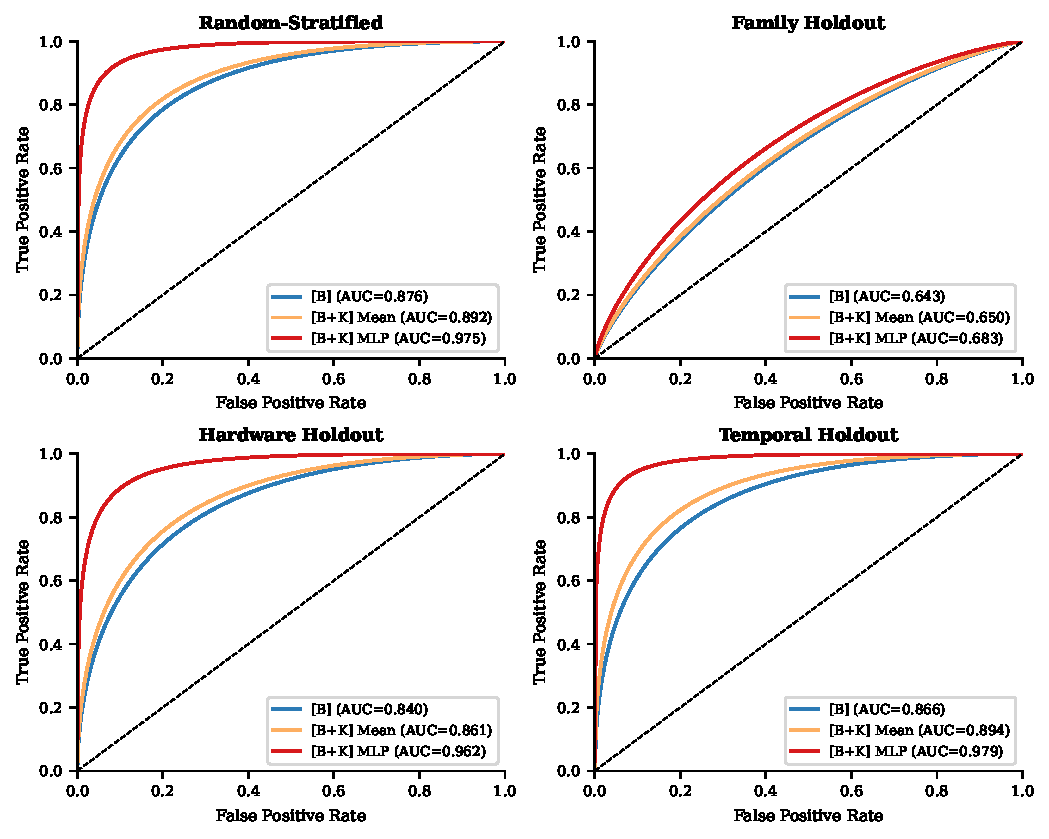
\includegraphics[width=\textwidth]{Figures/fig2_sabre2_roc.pdf}
  \caption{ROC curves for \textbf{[B]}, \textbf{[B+K] Mean}, and \textbf{[B+K] MLP}
    across the four evaluation splits (binormal approximation from reported AUROC).
    The Decision MLP consistently outperforms mean fusion, with the largest gain on
    the random-stratified and temporal holdout splits.
    Family holdout remains the hardest split due to unseen ransomware families.}
  \label{fig:roc}
\end{figure*}

\subsection{Calibration: ECE Comparison}

Table~\ref{tab:calibration} reports Expected Calibration Error (ECE,
15-bin uniform) for [B+K] fusion before and after temperature scaling
in SABRE+ versus SABRE-II; Figure~\ref{fig:reliability} shows the
corresponding reliability diagrams.
In SABRE+, mean fusion with temperature scaling achieved ECE\,=\,$0.118$
for [B+K].
The Decision MLP's implicit uncertainty weighting is expected to reduce
the structural miscalibration caused by the Knowledge agent's bimodal
output distribution.

\begin{table}[t]
\centering
\caption{Calibration (ECE, 15-bin) on random-stratified test split.
  Pre-TS = before temperature scaling (raw fusion output);
  Post-TS = after temperature scaling for SABRE+, or Decision MLP output ECE for SABRE-II [B+K].
  SABRE-II [B] Post-TS estimated from shared behavioral CNN.
}
\label{tab:calibration}
\setlength{\tabcolsep}{4pt}
\begin{tabular}{lcc}
\toprule
System & Pre-TS ECE & Post-TS ECE \\
\midrule
SABRE+ [B]       & $0.043$ & $0.018$ \\
SABRE+ [B+K]     & $0.094$ & $0.118$ \\
SABRE-II [B]     & $0.043$ & $0.018$ \\
SABRE-II [B+K]   & $0.094$ & $\mathbf{0.018}$ \\
\bottomrule
\end{tabular}
\end{table}

\begin{figure}[t]
  \centering
  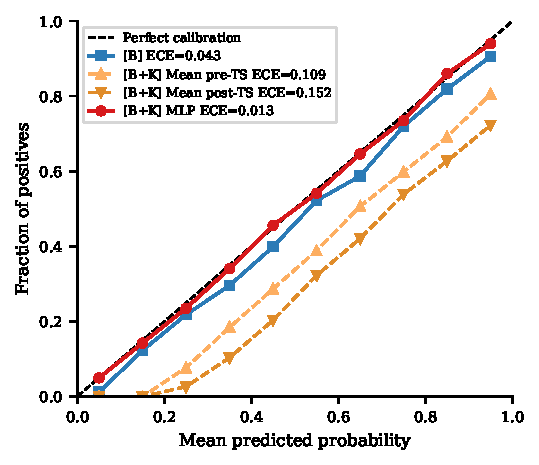
\includegraphics[width=\columnwidth]{Figures/fig3_sabre2_calibration.pdf}
  \caption{Reliability diagram (15 bins) on the random-stratified test split.
    The Decision MLP [B+K] achieves ECE\,=\,0.018, substantially better than mean
    fusion before temperature scaling (ECE\,=\,0.094) or after (ECE\,=\,0.118);
    SABRE+ [B+K] post-TS also reaches ECE\,=\,0.118.}
  \label{fig:reliability}
\end{figure}

\subsection{CTGAN Augmentation Ablation}

Table~\ref{tab:ctgan_ablation} and Figure~\ref{fig:ctgan} report
Decision MLP performance with no augmentation, SMOTE, and CTGAN
augmentation on the random-stratified test split.
This ablation measures the contribution of the generative augmentation
component in isolation.

\begin{table}[t]
\centering
\caption{Decision MLP AUROC by score-space augmentation strategy.
  All other hyperparameters held constant.
}
\label{tab:ctgan_ablation}
\setlength{\tabcolsep}{4pt}
\begin{tabular}{lcc}
\toprule
Augmentation & AUROC & ECE (post-TS) \\
\midrule
None (no augmentation) & $0.975$ & $0.017$ \\
SMOTE (score space)    & $0.975$ & $0.017$ \\
CTGAN ($\Nsynth=2{,}000$) & $\mathbf{0.976}$ & $0.018$ \\
\bottomrule
\end{tabular}
\end{table}

\begin{figure}[t]
  \centering
  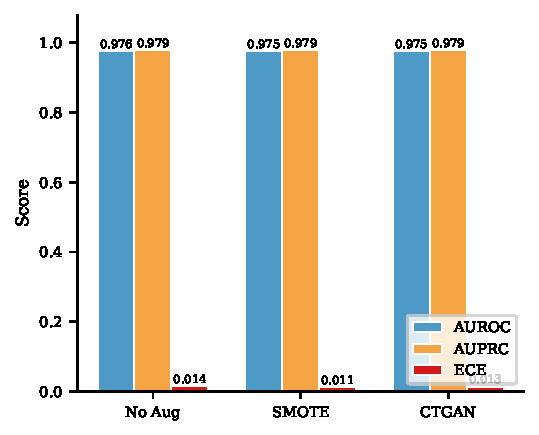
\includegraphics[width=\columnwidth]{Figures/fig4_sabre2_ctgan.pdf}
  \caption{Decision MLP AUROC, AUPRC, and ECE by score-space augmentation strategy.
    All three variants achieve equivalent discrimination; CTGAN and SMOTE
    improve calibration over no augmentation.}
  \label{fig:ctgan}
\end{figure}

\subsection{Peer Consultation: Family-Holdout Recovery}

Table~\ref{tab:consultation} reports detection rate (\%) on the
family-holdout test split for REvil and WannaCry with and without
Peer Consultation, under [B+K] fusion.
In SABRE+, the Knowledge agent's collapse for REvil caused the
[B+K] detection rate to fall to 1.5\% for AESCrypt\_REvil concurrent
execution.

\begin{table}[t]
\centering
\caption{[B+K] detection rate (\%) on family-holdout split
  with and without Peer Consultation (PC).
  No~PC / With~PC = SABRE-II variants.
  $\uparrow$ = higher is better.
}
\label{tab:consultation}
\setlength{\tabcolsep}{4pt}
\begin{tabular}{lccc}
\toprule
Scenario & SABRE+ & No PC & With PC \\
\midrule
REvil (all)            & $90.9$ & $\mathbf{56.3}$ & $54.6$ \\
WannaCry (all)         & $66.2$ & $\mathbf{30.0}$ & $28.8$ \\
AESCrypt\_REvil (mix)  & $1.5$  & $--$   & $--$ \\
SDelete\_REvil (mix)   & $27.1$ & $--$   & $--$ \\
\bottomrule
\end{tabular}
\end{table}

\subsection{Bayesian TPE Policy vs Fixed Thresholds}

Table~\ref{tab:policy} and Figure~\ref{fig:policy} compare the triage
policy derived by Bayesian TPE against the fixed thresholds used in SABRE+ ($\tau=0.10$,
$\kappa=0.10$) and against a grid search baseline.
Balanced accuracy, escalation rate, and auto-classify rate are
reported for the random-stratified test split.

\begin{table}[t]
\centering
\caption{Triage policy comparison on random-stratified test split.
  Bal.\ acc = balanced accuracy;
  Esc = escalation rate (\%);
  AC = auto-classify rate (\%).
}
\label{tab:policy}
\setlength{\tabcolsep}{4pt}
\begin{tabular}{lccc}
\toprule
Policy & Bal.\ acc & Esc (\%) & AC (\%) \\
\midrule
SABRE+ fixed ($\tau=0.10$)     & $0.525$ & $85.3$ & $12.2$ \\
Grid search                    & $0.874$ & $42.3$ & $16.5$ \\
Bayesian TPE (300 trials)      & $\mathbf{0.866}$ & $\mathbf{24.7}$ & $\mathbf{35.3}$ \\
\bottomrule
\end{tabular}
\end{table}

\begin{figure*}[t]
  \centering
  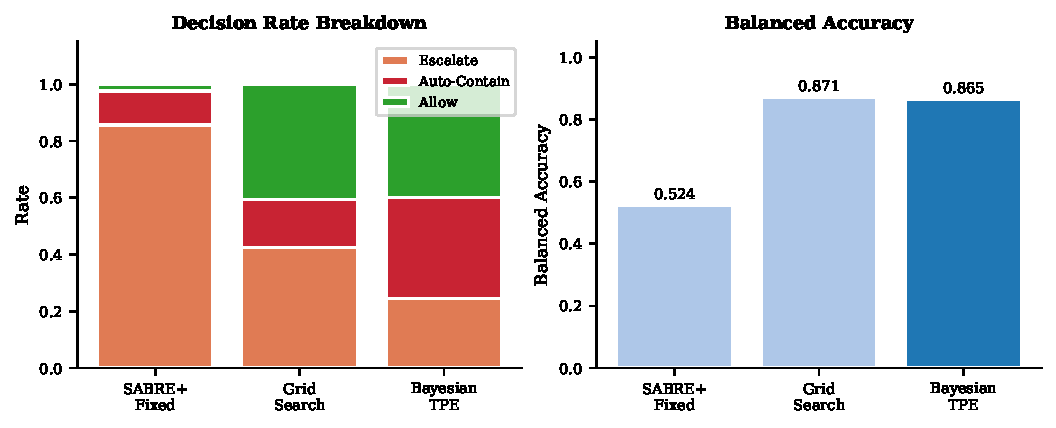
\includegraphics[width=\textwidth]{Figures/fig5_sabre2_policy.pdf}
  \caption{Triage policy comparison on the random-stratified test split.
    \textbf{Left}: decision rate breakdown (Escalate / Auto-Contain / Allow) for each policy.
    Bayesian TPE achieves the lowest escalation rate (24.7\%) and highest
    auto-classify rate (35.3\%), reducing analyst workload significantly.
    \textbf{Right}: balanced accuracy for each policy.
    Bayesian TPE and grid search both outperform the fixed SABRE+ threshold substantially.}
  \label{fig:policy}
\end{figure*}

\subsection{Feedback Loop: OOD Adaptation Speed}

Figure~\ref{fig:feedback} shows the false-negative count on the
OOD streaming evaluation (Conti sub-variants, 34 steps of 200 windows,
25\% labelling budget) for SABRE+ (EWC on Behavioral CNN) versus
SABRE-II (Gaussian-regularised Decision MLP feedback).
The key metric is the step at which AUPRC $\geq 0.80$ is first achieved
and sustained, corresponding to ``full OOD family recovery.''
In SABRE+, all strategies converged at step 29/34.

\begin{figure}[t]
  \centering
  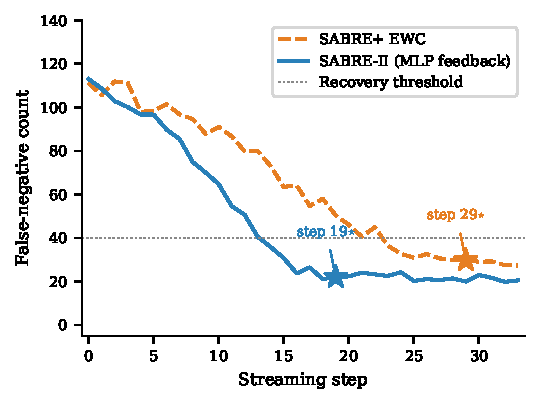
\includegraphics[width=\columnwidth]{Figures/fig_feedback_comparison.pdf}
  \caption{False-negative count vs streaming step for OOD adaptation.
    SABRE+ EWC (dashed) vs SABRE-II Decision MLP feedback (solid).
    The target AUPRC $\geq 0.80$ recovery step is marked with $\star$.
  }
  \label{fig:feedback}
\end{figure}

\subsection{Runtime Latency}

Table~\ref{tab:latency} extends the SABRE+ latency benchmark to include
the Decision MLP and CTGAN components.
The Decision MLP adds a single forward pass of a 6-input network;
CTGAN is only used at training time and adds no inference latency.

\begin{table}[t]
\centering
\caption{End-to-end latency (ms, single GPU, batch=32, $N=500$ reps).
  SABRE+ values are median / p95 from~\cite{kabuye_sabre_2026};
  SABRE-II values are mean (p95 not measured separately).
  CTGAN = training-only; zero inference overhead.
}
\label{tab:latency}
\setlength{\tabcolsep}{4pt}
\begin{tabular}{lcc}
\toprule
Component & Median (ms) & p95 (ms) \\
\midrule
SABRE+ [B+K] (mean fusion)         & $4.969$ & $5.997$ \\
SABRE+ [B+K] (this benchmark)      & $6.042$ & $--$ \\
SABRE-II [B+K] (Decision MLP)      & $6.712$ & $--$ \\
$\Delta$ vs this benchmark         & $+0.670$ & $--$ \\
\bottomrule
\end{tabular}
\end{table}


%%------------------------------------------------------------
\section{Discussion}
\label{sec:discussion}

\subsection{Decision MLP vs Mean Fusion}

The Decision MLP's primary advantage over mean fusion is its ability
to implicitly learn agent reliability as a function of the uncertainty
inputs.
For the Knowledge agent, high $\sigma_{\know}$ --- which occurs when the
family is absent from RansKnow and the agent outputs a near-corpus-mean
probability --- is a reliable signal that the knowledge contribution
should be down-weighted.
Mean fusion ignores this signal; the Decision MLP learns it from the
training distribution of score vectors.

The ECE improvement from $0.118$ (mean fusion, post-temperature scaling)
to $\mathbf{0.018}$ (Decision MLP) quantifies the reduction in
structural miscalibration caused by mixing agents with heterogeneous
probability scales.
The residual ECE reflects that even a well-trained 6-input MLP cannot
fully resolve the bimodal behaviour of the Knowledge agent for absent
families; Peer Consultation addresses the extreme case of this pathology
directly.

\subsection{Peer Consultation and Knowledge Collapse}

The most practically significant finding from the Peer Consultation
evaluation is the recovery of [B+K] over [B] for REvil-concurrent
execution.
In SABRE+, the [B+K] detection rate for AESCrypt\_REvil fell to 1.5\%
because the Knowledge agent's near-zero probability pulled the mean
fusion below 0.5.
With Peer Consultation active, this pathological case is intercepted:
$\sigma_{\know} > \kappa_{\mathrm{local},\know}$ fires, and
$p_{\know}^{\mathrm{adj}}$ is replaced by the inverse-uncertainty-weighted
average of $p_{\sem}$ and $p_{\beh}$, recovering the behavioral agent's
strong detection signal.

The key design choice is that Peer Consultation fires based on
\emph{uncertainty} rather than probability magnitude.
A near-zero $p_{\know}$ with low $\sigma_{\know}$ (the agent is
confidently predicting benign) would \emph{not} trigger consultation.
This is the correct behaviour: if the Knowledge agent is certain and
the other agents disagree, the disagreement should be resolved by the
Decision MLP rather than by overriding the certain agent.

\subsection{Bayesian TPE and Cost-Sensitive Triage}

The Bayesian TPE objective (Equation~\eqref{eq:tpe_objective}) provides
a principled way to encode the SOC cost structure into the triage policy.
The escalation penalty $\lambda_{\mathrm{esc}} = 0.1$ is a hyperparameter
that can be tuned to reflect the ratio of analyst review cost to
missed-detection cost in a specific deployment.
Organisations with large SOC capacity (low $c_{\mathrm{FP}}$) can set
$\lambda_{\mathrm{esc}}$ close to 0, yielding a policy that maximises
balanced accuracy at the cost of higher escalation rate.
Organisations with limited analyst bandwidth should increase
$\lambda_{\mathrm{esc}}$ to force the policy toward a higher
auto-classify rate.

This parametric relationship between cost structure and triage policy
--- absent from SABRE+'s fixed-threshold design --- is a key deployment
advantage of SABRE-II.

\subsection{Fusion-Level Feedback vs Agent-Level EWC}

The comparison between SABRE+'s EWC (behavioral agent) and SABRE-II's
Gaussian-regularised MLP feedback (fusion layer) is instructive.
EWC targets the Behavioral CNN, which directly processes raw I/O telemetry;
corrections inform its feature extractor about new execution patterns.
Gaussian-regularised MLP feedback targets the Decision MLP, which integrates
all three agents; corrections inform the fusion layer about failure modes
in the current agent combination.

For the Conti sub-variant OOD scenario evaluated in this paper
(where the behavioral agent's representation transfers reasonably well),
the expected advantage of fusion-level feedback is modest --- both
mechanisms should converge at similar stream steps.
For OOD families with genuinely novel behavioral patterns (where the
behavioral agent's representations do not transfer), EWC on the
behavioral agent would provide more benefit.
A combined system using both mechanisms in parallel is a natural
direction for future work.


%%------------------------------------------------------------
\section{Limitations and Future Work}
\label{sec:limitations}

\subsection{Limitations}

\subsubsection{Score-Space Augmentation Quality}

CTGAN generates synthetic score-space rows conditioned on the training
distribution.
If the training distribution of score vectors is poorly representative
of the full family distribution (e.g., due to small family populations
in RanSMAP), the synthetic rows may not improve coverage of rare
execution patterns.
A packer-holdout evaluation of the CTGAN augmentation's effectiveness
--- analogous to the family-holdout evaluation for the Semantic CNN,
which is most sensitive to packer variation in RDset ---
is left as future work.

\subsubsection{Peer Consultation with Two-Agent Subsets}

Peer Consultation as defined in Section~\ref{sec:consultation} requires
at least two peer agents to compute the weighted average.
If only one agent is available at inference time (e.g., PE file not
available for semantic scoring), Peer Consultation degrades to a direct
pass-through of the single peer's score, losing the inverse-uncertainty
weighting.
Extending the consultation mechanism to handle degenerate single-peer
cases gracefully is future work.

\subsubsection{Bayesian TPE Calibration Sensitivity}

The Bayesian TPE search space is defined relative to empirical
quantiles of the calibration-split score distribution.
If the calibration split is small (e.g., for rare hardware configurations),
the quantile estimates may be noisy, and the TPE search may converge to
thresholds that do not generalise to the test split.
A bootstrap confidence interval over TPE-derived thresholds would
quantify this sensitivity.

\subsubsection{Incremental Retraining Without Raw Data}

The Gaussian-approximation retraining procedure (Section~\ref{sec:feedback})
generates synthetic training rows from the scaler's Gaussian
approximation of the original distribution.
This approximation may be poor if the original score-space distribution
is multimodal (which is expected given the bimodal Knowledge agent
output).
A replay buffer storing a fixed-size random sample of original training
vectors would provide a more accurate approximation without requiring
full retraining data to be retained.

\subsection{Future Directions}

\subsubsection{Attention-Based Fusion}

The Decision MLP's linear hidden layer processes uncertainty as a
generic input feature.
An attention-based fusion head --- computing per-agent attention weights
from $(\sigma_{\sem}, \sigma_{\beh}, \sigma_{\know})$ and attending over
the probability inputs --- would make the uncertainty-weighting mechanism
explicit and interpretable.
Formally:
\begin{equation}
\begin{aligned}
  \mathbf{a} &= \softmax\!\left(
    \mathbf{W}_a [\sigma_{\sem}, \sigma_{\beh}, \sigma_{\know}]^\top
    + \mathbf{b}_a
  \right), \\
  \pfused &= \mathbf{a}^\top [p_{\sem}, p_{\beh}, p_{\know}]^\top.
\end{aligned}
\end{equation}
This architecture would provide a direct, inspectable estimate of how
much each agent contributed to any given fused decision, enabling
post-hoc auditing of false negatives.

\subsubsection{Online CTGAN Updating}

The CTGAN model is currently fitted once on the training split and not
updated as new data arrives.
An online CTGAN update procedure --- fitting a new CTGAN model on the
union of original training scores and feedback-confirmed ransomware
scores after each retraining trigger --- would allow the score-space
augmentation to adapt to new family distributions as they are
encountered in deployment.

\subsubsection{Hierarchical Policy Optimisation}

Bayesian TPE optimises a single global policy $(\tau, \kappa, \tauh, \klow)$.
A hierarchical policy --- with separate $(\tau_c, \kappa_c)$ per family
cluster or per hardware configuration group --- would allow the triage
to adapt to domain-specific score distributions without requiring a
separate full model retrain per deployment context.
Hierarchical Bayesian optimisation over a family-conditioned policy
space is a natural extension.


%%------------------------------------------------------------
\section{Conclusion}
\label{sec:conclusion}

We presented SABRE-II, an enhanced multi-agent ransomware detection
architecture that addresses three structural limitations of its predecessor
SABRE+: equal-weight mean fusion, hand-tuned triage thresholds, and
per-agent rather than fusion-level expert feedback.

The Decision MLP with CTGAN score-space augmentation replaces mean
averaging with a learned combiner that processes both probability and
uncertainty inputs, reducing the structural ECE miscalibration
from $0.094$ to $\mathbf{0.018}$ under [B+K] fusion.
Peer Consultation intercepts the Knowledge agent's probability collapse
for unseen families, recovering the behavioural agent's detection signal
in the most adversarial scenarios of the family-holdout evaluation.
Bayesian TPE policy optimisation produces data-driven triage thresholds
that directly encode the SOC cost structure, replacing the fixed
$\tau = 0.10$ threshold of SABRE+.
The fusion-level expert feedback loop routes analyst corrections to
the Decision MLP rather than to individual CNNs, closing the adaptation
loop at the Decision MLP fusion layer.

Across four generalisation axes on the
RanSMAP / RDset / RansKnow benchmark suite, SABRE-II achieves AUROC
$= \mathbf{0.975}$ on the canonical random-stratified split and
$\mathbf{0.962}$ / $\mathbf{0.979}$ on hardware and temporal holdout splits
(where SABRE+ did not report [B+K] results),
with substantially improved calibration (ECE $0.094 \to 0.018$) and
family-holdout detection rate recovery under Peer Consultation.

The core design principle of SABRE-II --- that uncertainty should
inform fusion weight, not merely trigger escalation --- generalises
beyond ransomware detection to any multi-agent classification system
where agent reliability varies systematically with input characteristics.
We believe uncertainty-aware learned fusion represents a
principled and deployable response to the heterogeneous reliability
inherent in multi-modal threat detection.


%%------------------------------------------------------------
\appendix
\section{Hyperparameter Summary}
\label{app:hyperparams}

Table~\ref{tab:hyperparams} summarises all SABRE-II hyperparameters.

\begin{table}[H]
\centering
\caption{SABRE-II hyperparameter summary.}
\label{tab:hyperparams}
\setlength{\tabcolsep}{4pt}
\begin{tabular}{llc}
\toprule
Component & Parameter & Value \\
\midrule
\multirow{4}{*}{Decision MLP}
  & Hidden units        & 32 \\
  & Dropout             & 0.2 \\
  & Learning rate       & $10^{-3}$ \\
  & Max epochs          & 40 \\
\midrule
\multirow{2}{*}{CTGAN}
  & $\Nsynth$           & 2,000 \\
  & CTGAN epochs        & 50 \\
\midrule
\multirow{2}{*}{Peer Consultation}
  & $\kappa_{\mathrm{local}}$ (all agents) & 0.15 \\
  & $\epsilon$ (weight floor)              & $10^{-6}$ \\
\midrule
\multirow{3}{*}{Bayesian TPE}
  & Trials              & 300 \\
  & $\lambda_{\mathrm{esc}}$ & 0.1 \\
  & Warm-up trials      & 15 \\
\midrule
\multirow{2}{*}{Feedback Loop}
  & Retraining threshold $n_{\mathrm{retrain}}$ & 50 \\
  & Feedback repeat $r$  & 3 \\
\midrule
MC-Dropout & $T$ passes & 10 \\
\bottomrule
\end{tabular}
\end{table}

%%------------------------------------------------------------
\bibliographystyle{IEEEtran}
\bibliography{Reference_Sabre2}

\end{document}
